% Required packages: texlive-bibtex-extra

\documentclass[10pt, oneside, letterpaper]{article}
\usepackage[utf8]{inputenc}

\usepackage{authblk}
	\setcounter{Maxaffil}{0}
	\renewcommand\Affilfont{\itshape\small}
\usepackage{float}
\usepackage[margin=1.5in]{geometry}
\usepackage{graphicx}
	\graphicspath{ {img/} }
\usepackage[colorlinks=true, linkcolor=blue, urlcolor=blue, citecolor=blue]{hyperref}
\usepackage{indentfirst}
\usepackage{multicol}
\usepackage{ragged2e}
\usepackage{verbatim}

% Second set of package loads
\usepackage{apacite}  % Must occur after hyperref

\title{\textbf{The Capabilities of Microelectrodes}}
\author{Jeffrey Leung}
\affil{Simon Fraser University}
\date{February 09, 2015}

\begin{document}

	\maketitle

	\begin{abstract}
		This paper is an assignment for IAT 267: Introduction to Technological Systems. The material construction and technical capabilities of a microelectrode are examined. Current and future applications in human enhancement technology are discussed.
	\end{abstract}

	\begin{multicols}{2}

	Human bodies have changed and adapted over hundreds of thousands of years, from lean hunter-gatherers who raced tirelessly over long distances to exhaust their prey to perfectly-sculpted athletes who run faster, work harder, and are stronger than any other human before our time. Every day, humanity redefines the limits of what we originally thought possible. However, what if the next significant step in our adaption is not biological, but mechanical? Is it possible for us to mechanically augment our bodies and minds to push the limits beyond what is biologically possible? To do this, a neural connection will be required for us to send commands and receive information from machines, literally at the speed of light. The key to this neural connection is a microelectrode sensor.

	\begin{figure}[H]
		\centering
		\href
			{http://deusex.wikia.com/wiki/File:CyberneticArmProsthesis2.png}
			{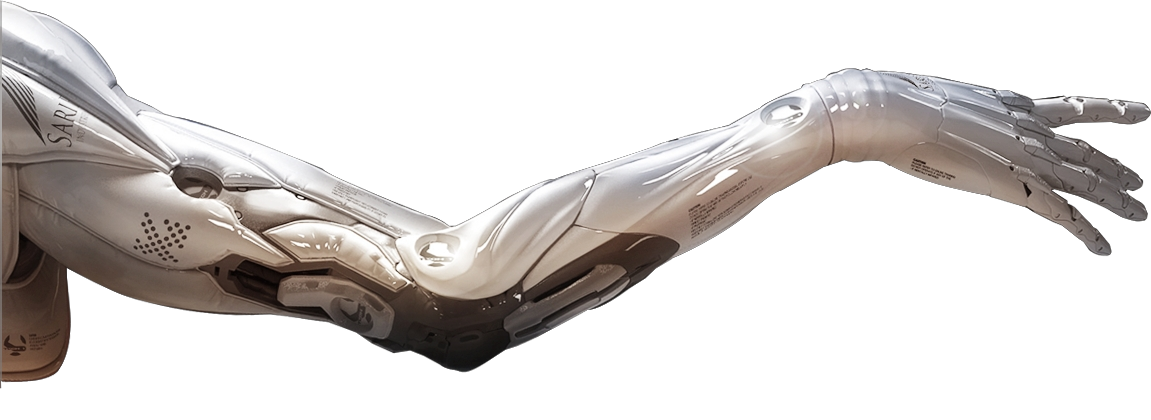
\includegraphics[width=\linewidth]{cybernetic-arm-prosthesis}}
		\caption{Conceptual Cybernetic Arm Prosthesis \protect\cite{Eidos2011}}
		\label{fig:cybernetic-arm-prosthesis}
	\end{figure}

	To define the term `microelectrode', we must first determine what an electrode is. An \emph{electrode} is an electrical conductor which conveys electrical signals to and/or from a material. Genrally, electrodes can be any size. A \emph{microelectrode} is an electrode which is incredibly small - for example, its tip may be several micrometers in diameter, or even possibly under a micrometer in some biological applications. They are often used for sensitive measurements in small, difficult to reach locations. When implanted into a biological entity, microelectrodes are designed to be minimally intrusive and damaging through their size and material. See figure~\ref{fig:redox-microelectrode} for a picture of a microelectrode.

	\begin{figure}[H]
		\centering
		\href
		{http://www.unisense.com/Redox}
		{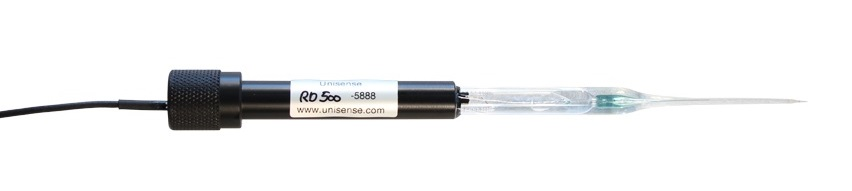
\includegraphics[width=\linewidth]{redox-electrode}}
		\caption{Picture of a Redox Microelectrode \protect\cite{Unisense}}
		\label{fig:redox-microelectrode}
	\end{figure}

	The purpose of a microelectrode is to detect electrical impulses (if used as an input sensor) or to send electrical signals (if used as an output transducer). When connected to biological tissue, the microelectrode may be pierced into a cell without damaging it, in order to be able to collect or send information without issue. As an input sensor, electrical potential is measured directly; however, the measurement can also be used to calculate how much of a chemical is emitted by the body at any given time, using the resistance of the chemical \cite{Boccaletti2008}, \cite[p.~453]{Montenegro1991}. As an output transducer, the microelectrode may act as a neurostimulator (signal sent by the brain to control the body) in lieu of the body's nervous impulses.

	Due to the numerous possible applications of microelectrodes, there are many different possible ways to manufacture a microelectrode. A voltammetric electrode consists of metallic terminals between which an external voltage is sent, and the result is measured \cite{BASinc}. A potentiometric electrode may either consist of a glass tube or a membrane. Within the glass tube is either a solution or a wire made from an inert metal such as platinum or gold \cite{McMahon2016}. Both the glass tube and membrane are used to measure potential difference, between multiple glass tubes or across two points of the membrane. See figure~\ref{fig:glass-microelectrode} for a diagram of a glass microelectrode. Essentially, a microelectrode can measure electrical potential in a material using capacitance (the electrical energy stored by an object). There are many more subtle details on how microelectrodes function physically due to electron transfer and simultaneous chemical reactions, but the main emphases are that the electrode is a receptacle of electrons, and it must be chemically inert.

	\begin{figure}[H]
		\centering
		\href
		{http://www.intechopen.com/books/microsensors/a-glass-capillary-based-microsensor-for-l-glutamate-in-in-vitro-uses}
		{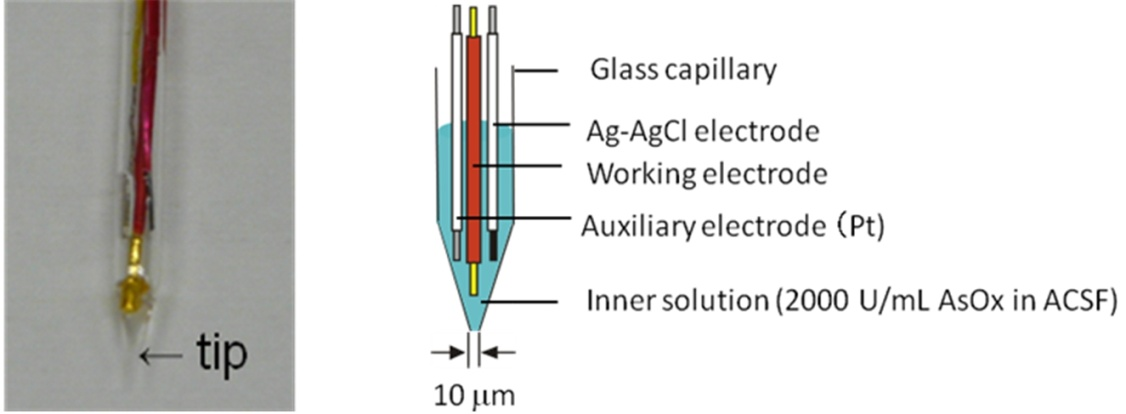
\includegraphics[width=\linewidth]{glass-capillary-microelectrode}}
		\caption{Diagram of a Glass Microelectrode \protect\cite{Suguwara2011}}
		\label{fig:glass-microelectrode}
	\end{figure}

	As a sensor, a microelectrode works very similarly to a capacitor by measuring capacitive potential and potential difference and outputting a variable voltage. This variable voltage can then be analyzed to determine the amount of electrical potential in the space around the microelectrode. Microelectrodes must be extremely precise (i.e. little to no variability between distinct microelectrodes) in their physical composition to ensure repeatable and consistent measurements, and they must also be extremely sensitive (able to detect miniscule changes) due to the necessity of detecting subtle changes in a biological system.

	As explained above, a microelectrode can be designed like a capacitor to measure potential difference. In a circuit, the two terminals of the microelectrode would be connected to the anode and cathode, similar to most simple electrical components. See figure~\ref{fig:example-schematic-biopotential-electrode} for an example schematic of a microelectrode in a circuit \cite{Boccaletti2008}. When used in the brain to detect neural signals, microelectrodes are often arranged in an array for greater coverage and accuracy (i.e. a closer overall measurement of the actual value). \citeA{McMahon2016} mentions the use of microelectrode arrays for cybernetic prostheses, and \citeA{Sonn1974} describe ways to create a plastic array of platinum microelectrodes implanted in the brain to allow for a cochlear implant. Placement is also a key issue, as \citeA{Stoller2015} found that placing microelectrodes closer to the location in the brain where the intention of an action originates is more effective. For example, placing the microelectrode in the brain area where the subject creates the intention to move their arm tends to be more effective than placing the microelectrode in the brain area where the subject creates details about how to move their arm. Today, we are still learning a great deal about how to retrieve signals from and send signals into the brain.

	\begin{figure}[H]
		\centering
		\href
		{http://www.biophysics-research.com/Validazione.aspx}
		{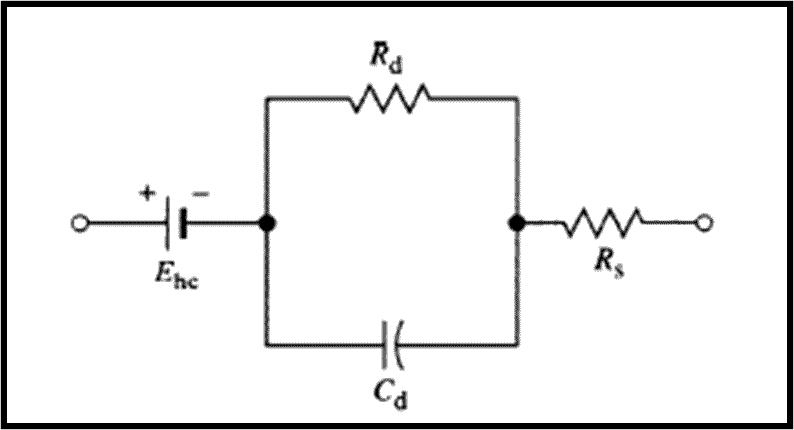
\includegraphics[width=\linewidth]{circuit-biopotential-electrode}}
		\caption{Example Schematic of a Biopotential Electrode \protect\cite{Boccaletti2008}}
		\label{fig:example-schematic-biopotential-electrode}
	\end{figure}

	Commercially, microelectrodes are allowing for incredible developments in removing a physical barrier of interaction with our world. When used as detectors in the body, microelectrodes can measure the amount of oxygen in biological tissue \cite[p.~454]{Montenegro1991}. Some carbon-fiber microelectrodes allow detection of the presence and amount of a neurotransmitter, a chemical produced by the body which conveys messages, such as dopamine  \cite[p.~453]{Montenegro1991}.

	Possibly the most fascinating purpose of a microelectrode system, however, would be to replace or augment current human biological features. For example, cochlear and retinal implants may be able to use microelectrodes to send input directly into the brain, therefore allowing a complete replacement of a damaged auditory or visual system. \citeA{Knapton2016} discusses a brain-damaged musician who was able to use an electrode cap to create music, which was played live by musicians. As well, entire limbs can be simulated solely using neural signals, such as in the case of a quadriplegic patient (loss of control of all 4 limbs) who was able to use a robotic arm naturally and easily, simply through neural microelectrodes \cite{Stoller2015}.

	Given that microelectrodes are our key to tapping directly into the brain, we are able to create neurally-controlled machines which interact with the environment in increasingly versatile and powerful ways. If microelectrodes can be used to breach the barrier between a natural and intuitive brain-machine interface (the direct control of machines through neural signals), then what will we be be able to engineer to improve upon human capabilities and break through biological limits? Perhaps we will create a device which can speak words directly from our thoughts \cite{Knapton2014}. Perhaps we will design an additional retinal sensor which will allow us to see a far greater colour spectrum than we can with our natural eyes \cite{Classroom}. Perhaps we will be able to control robots remotely with immense precision. Perhaps we will achieve the near-perfect neural control of mechanical prostheses which will completely replace lost human limbs.

	In our next step of human evolution, we are limited only by our imaginations.

	\begin{figure}[H]
		\centering
		\href
		{http://deusex.wikia.com/wiki/File:SarifIndustriesMainPage.png}
		{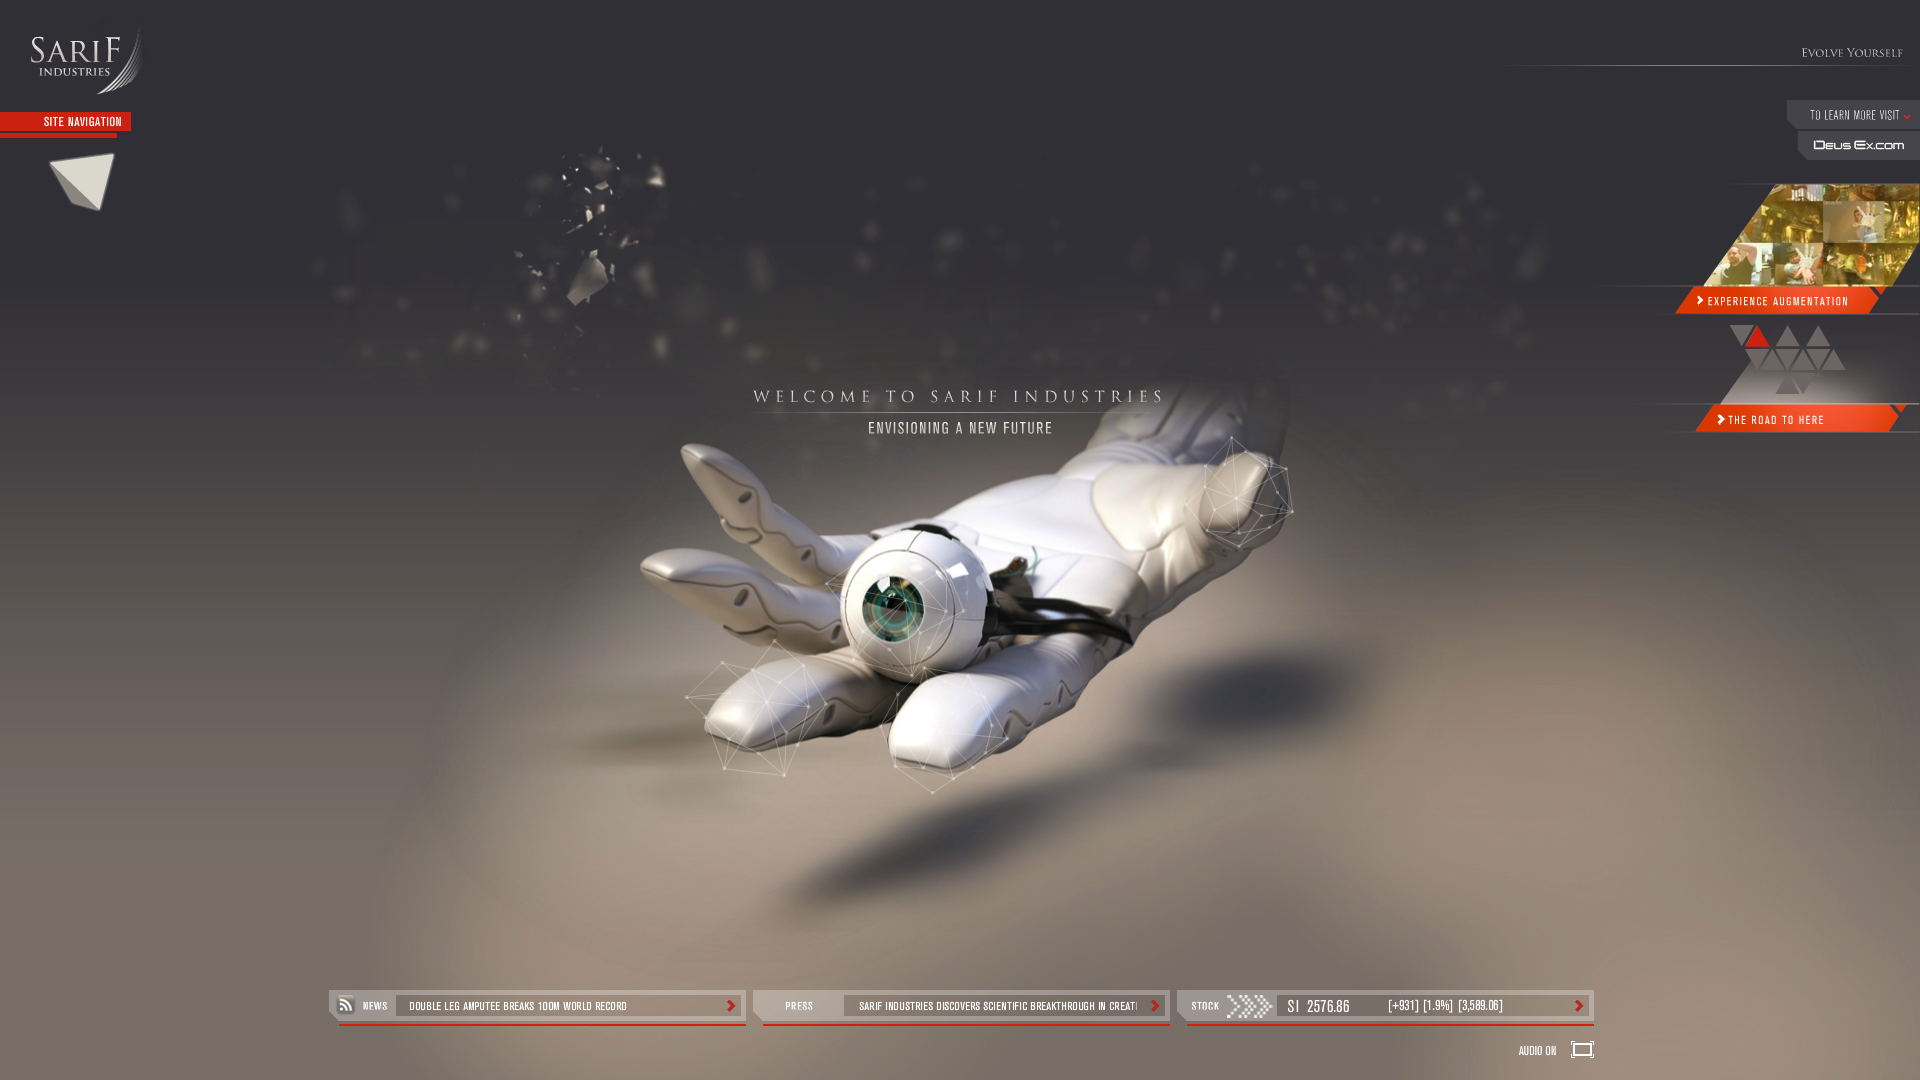
\includegraphics[width=\linewidth]{sarif-industries-main-page}}
		\caption{Website of a Fictional Technological Development Corporation \protect\cite{Eidos2011}}
	\end{figure}

	\begin{figure}[H]
		\centering
		\href
		{https://youtu.be/lc3Bzkgkbzg?t=1m57s}
		{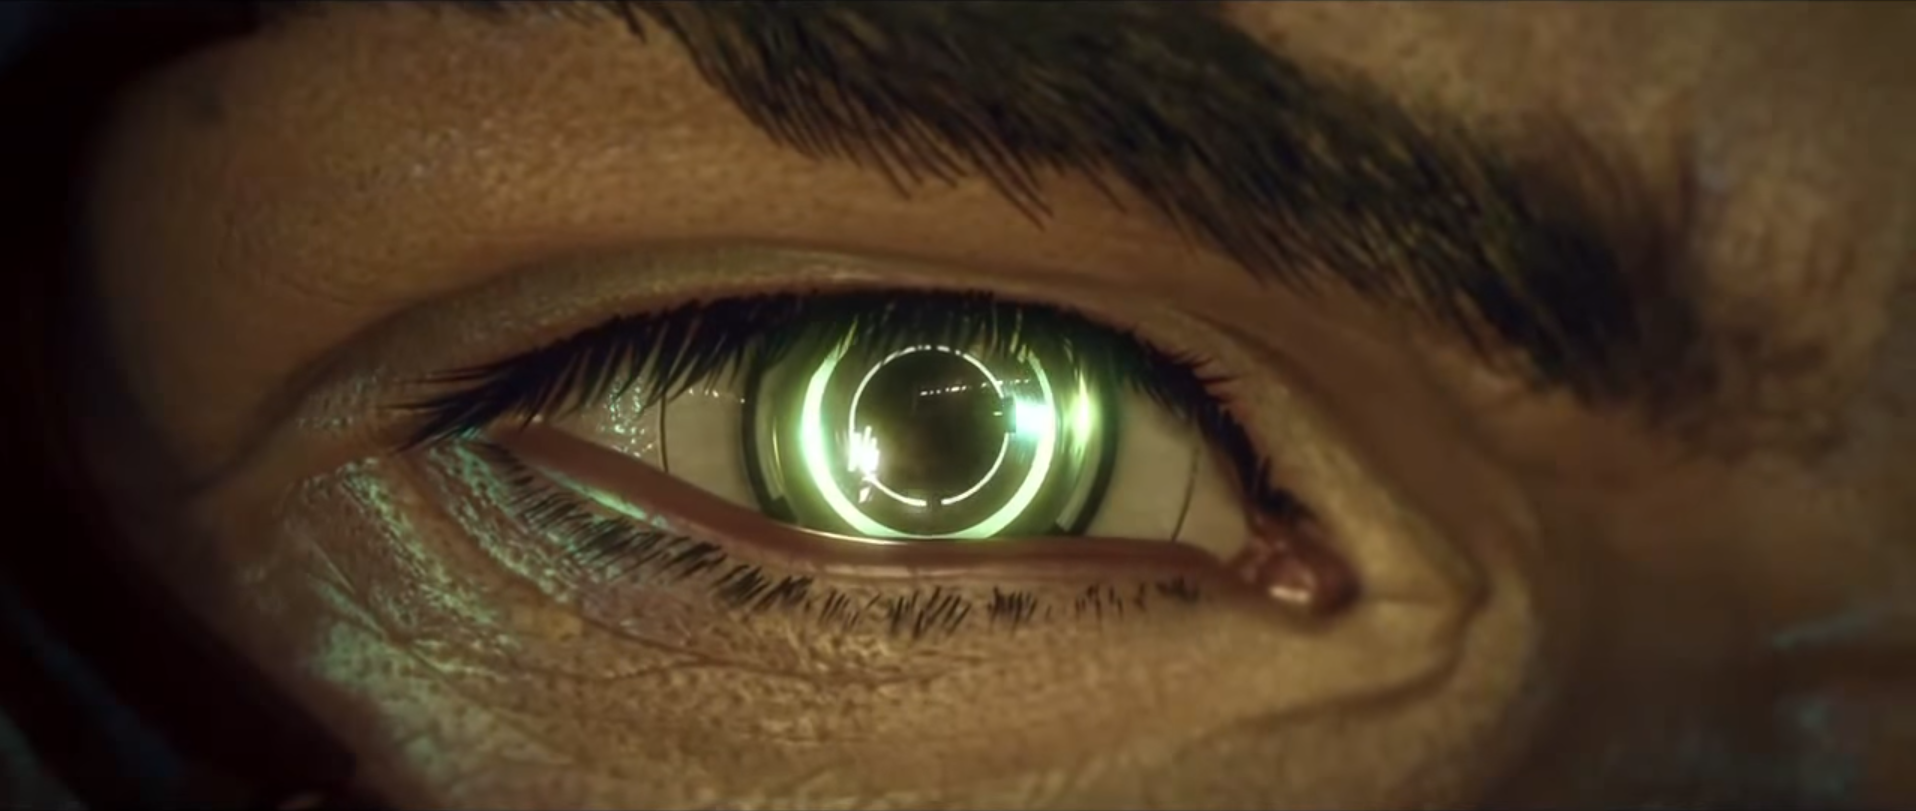
\includegraphics[width=\linewidth]{adam-jensen-eye}}
		\caption{Augmented Eye \protect\cite{Eidos2011}}
	\end{figure}

	\end{multicols}

	{\RaggedRight
		\bibliographystyle{apacite}
		\bibliography{capabilities-of-microelectrodes}
	}

\end{document}